\setlength{\footskip}{8mm}

\chapter{LITERATURE REVIEW}\label{literatureReview}

We review the result of Raman spectra of amorphous glucose (glucose fingerprint) when combined with water (glucose solution) and blood (blood glucose). 
Then, we go into measuring sites and preprocessing techniques, and data modeling.

% \section{Measuring Glucose in blood}

% Measured Raman signal can be seen as four parts \cite{directGlucose}. 
% (1) glucose Raman spectrum (G), (2) tissue (non-glucose) Raman spectrum (T), (3) time-varying tissue background signal ($B_T$), and (4) time-independent system background signal ($B_S$).
% Glucose signals changes according to the amount of glucose that exists in the blood. 
% This means $\Delta G = G_{t_1} - G_{t_2}$ where $G_{t_1}$ and $G_{t_2}$ is glucose signal at time $t_1$ and $t_2$ respectively.
% Tissue Raman is generated by lipids, proteins, and collagen. 
% When measuring the same spot, the tissue Raman stays relatively unchanged.
% This means $\Delta T = T_{t_1} - T_{t_2} \approx 0$.
% For time-varying tissue background and time-independent system background, the difference at two-time points is $\Delta B_T = B_{T_{t_1}} - B_{T_{t_2}}$ and $\Delta B_S = B_{S_{t_1}} - B_{S_{t_2}}$.
% Given the $\Delta t$ is small, $\Delta B_T$ and $\Delta B_S$ is $\approx 0$.

% The Raman signal ($R$) consists of four parts that can be modeled as $R = G + T + B_T + B_S$.
% Then, the $\Delta R$ would be $\Delta G + \Delta T + \Delta B_T + \Delta B_S$.
% It is obvious that, given $\Delta t$ is small, the $\Delta R = \Delta G + 0 + 0 + 0 = G_{t_1} - G_{t_2}$.




%%%%%%%%%%%%%%%%%%%%%%%%%%%%%
\section{Glucose fingerprint}

\begin{figure}
    \caption{Raman spectra of glucose solution at different concentration \citep{solutionGlucose}.}
    \centerline{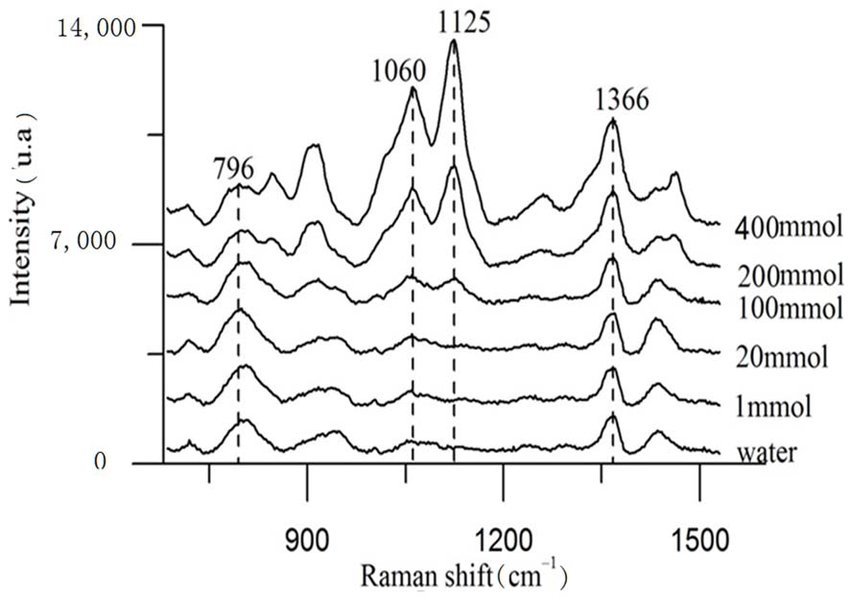
\includegraphics[width=3in]{figures/solutionGlucose-RS.jpg}} \label{fig:solutionGlucose-RS}
    % \small{\textit{Note.} Additional notes goes here.}
\end{figure}

\begin{figure}
    \caption{A trace of glucose fingerprint in Raman scattering of in vivo blood \citep{solutionGlucose}.}
    \centerline{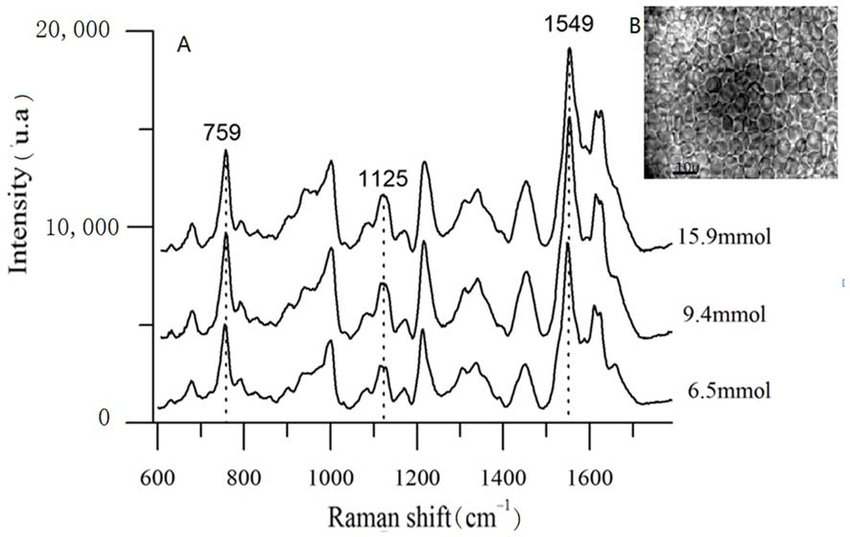
\includegraphics[width=3in]{figures/bloodGlucose-RS-2012.jpg}}\label{fig:bloodGlucose-relative1125}
    % \small{\textit{Note.} Additional notes goes here.}
\end{figure}

The ``glucose fingerprint'' is a characteristic Raman scattering spectrum that appears when glucose is present in the analyte.
The Raman scattering in glucose solution (glucose and water) exhibits peaks at 796, 1060, 1125, and 1366 $\text{cm}^{-1}$ (Figure~\ref{fig:solutionGlucose-RS}).
These peaks increase as a function of glucose concentration showing the quantitative property of Raman spectroscopy \citep{solutionGlucose}.
The glucose fingerprint also exhibits in a more complex analyte as blood when measuring Raman scattering of ISF \citep{forearm2005, forearm2014, directGlucose, sitecompare} as show in Figure~\ref{fig:bloodGlucose-relative1125}.

\begin{figure}
    \caption{(\textbf{A}) Raman spectra of blood glucose obtained by subtracting two Raman signals \citep{directGlucose}.}
    \centerline{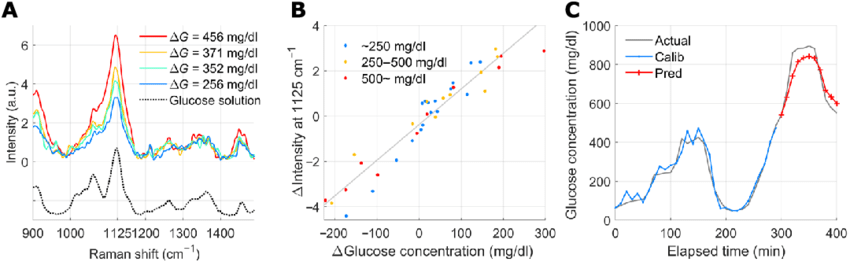
\includegraphics[width=3in]{figures/bloodGlucose-DeltaG.png}}\label{fig:bloodGlucose-DeltaG}
    % \small{\textit{Note.} Additional notes goes here.}
\end{figure}

\cite{directGlucose} extracts the glucose fingerprint which has a peak at 1125 $\text{cm}^{-1}$ from two noisy Raman signals.
As a result, Raman spectroscopy can measure blood glucose.



\begin{table}[]
\caption{Assignments of Raman peaks that are identified in the spectra of the microvessels and blood \citep{peak45,forearm2005,peak47,peak48}}
\begin{center}
\begin{tabular}{cccc}
\hline
\multicolumn{2}{l}{Peak Position ($\text{cm}^{-1}$)} & \multirow{2}{*}{Assignments}  & \multirow{2}{*}{Components} \\ \cline{1-2}
Microvessels         & Blood         &                               &                             \\ \cline{1-2}
\hline
650                  & 643           & P:C-S str                     & Ascorbic acid               \\
758                  & 752           & $\nu_{15}$                    & Trp                         \\
837                  & 827           & $\gamma10$                    & Fructose                    \\
858                  & 855           & $\nu(C-C)$                    & Tyr, lac                    \\
885                  & -             & -                             & -                           \\
902                  & 898           & p:C-C skeletal                & Tyr                         \\
945                  & 940           & $\nu(C-C)$                    & Crtic acid                  \\
978                  & 971           & p: Skeletal vibr              & Fibrin                      \\
1004                 & 1004          & $\nu$-ring                    & Phe                         \\
1027                 & 1026          & $\delta(={C}_{b}{H}_{2})$asym & Lac                         \\
1130                 & 1129          & $\nu_5$,                      & Lac                         \\
1163                 & 1157          & $\nu_{44}$                    & Heme                        \\
1217                 & 1212          & $\nu_5 + \nu_{18}$            & Heme                        \\
1320                 & 1321          & p: CH2 twist                  & Try                         \\
1332                 & 1341          & $\nu_{41}$                    & Trp                         \\
1424                 & 1423          & $\nu_{28}$                    & Acetates                    \\
1448                 & 1450          & $\delta(={CH}_{2}/{CH}_{3})$  & Trp                         \\
1551                 & 1546          & $\nu_{11}$                    & Heme                        \\
1608                 & 1603          & $\nu(C=C)_{\text{venyl}}$     & Heme                        \\
1660                 & 1653          & Amide I                       & Heme                        \\
\hline
\end{tabular}
\label{tab:bloodpeak}
\end{center}
\end{table}





% This same phenomena occur when measuring Raman scattering of blood glucose in vivo \citep{forearm2005, forearm2014, directGlucose, sitecompare}.
% In \cite{directGlucose}, after subtracting the two Raman spectra measure at two different time points, the spectra peaks at 1125 $\text{cm}^{-1}$.
% Unlike the glucose solution, Raman signal of blood is noisy because of blood contains various substance \citep{ramanNailFold2019}.
% To extract the linearity relationship, the 1125 $\text{cm}^{-1}$ has to be normalized with the peaks of protein and lipid (1450 $\text{cm}^{-1}$ \citep{directGlucose}, 1549 $\text{cm}^{-1}$ \citep{solutionGlucose}).

\section{Measuring Sites}

% Laser can penetrate the skin around $100 - 200 \mu\text{m}$
Because the thickness of the human skin varies from place to place, Raman scattering measurements taken at several sites might provide varied results \citep{ramanNailFold2019, sitecompare}.
The glucose fingerprint signal will be stronger if the laser focuses on the blood vessels \citep{solutionGlucose}.
Human skin consists of multiple layers called the stratum corneum (SC), epidermis, and dermis \citep{ramanNailFold2019}.
In most sites (e.g., wrist, forearm, fingertip), the assessed Raman signal is from ISF of SC and epidermis layer \citep{ramanNailFold2019}.
The following problems may arise when measuring glucose in ISF rather than blood, 
(1) ISF glucose is lag when compared to blood glucose \citep{bloodvsisf, isflag}, 
(2) concentration of glucose in ISF is significantly lower than blood \citep{isfconcentration}. 
As a result, the signal of glucose Raman scattering is weak \citep{ramanNailFold2019}.
A better strategy is to measure the Raman signal in areas where the laser can reach the dermis better.
Because the dermis contains microvessels \citep{microvessel-dermis, microvessel-dermis2}, if the site (nailfold) is picked carefully, we can obtain the glucose signal directly from the blood.

\cite{ramanNailFold2019} reports the greater $R^2 = 0.98$ prediction correlation when use nailfold as a measuring site.
The result is better than the forearm ($R^2 = 0.83$) \citep{forearm2005,forearm2014} and fingertip ($R^2 = 0.91$) \citep{fingertip2011}.
Recently, \cite{sitecompare} measures Raman glucose at forearm, wrist, and index fingertip and achieves the root-mean-square error (RMSE) of $56.31\pm4.28$, $58.22\pm1.03$, and $56.65\pm8.99$ ml/dL respectively.

\section{Preprocessing techniques and Data modeling}

\begin{figure}
    \caption{(\textbf{A}) Blood glucose value with 1125 $\text{cm}^{-1}$ relative intensity. (\textbf{B}) Concentration-dependent Raman relative intensities of glucose (1125 $\text{cm}^{-1}$) \citep{solutionGlucose}}
    \centerline{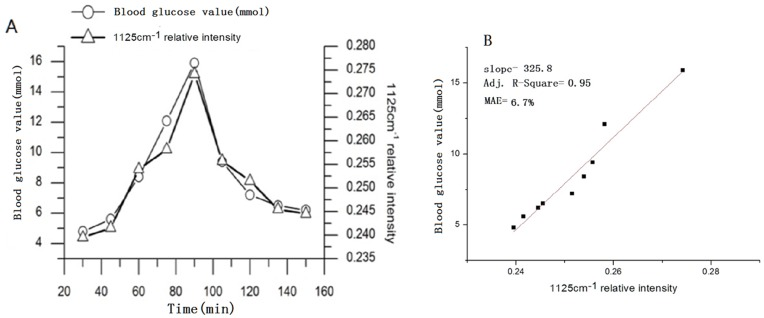
\includegraphics[width=3in]{figures/bloodGlucose-relative1125.png}}\label{fig:bloodGlucose-relative1125}
    % \small{\textit{Note.} Additional notes goes here.}
\end{figure}

\begin{figure}
    \caption{(\textbf{B}) Showing the linear relationship between normalized 1125 $\text{cm}^{-1}$ with blood glucose ($R^2 = 0.94$) \citep{directGlucose}}
    \centerline{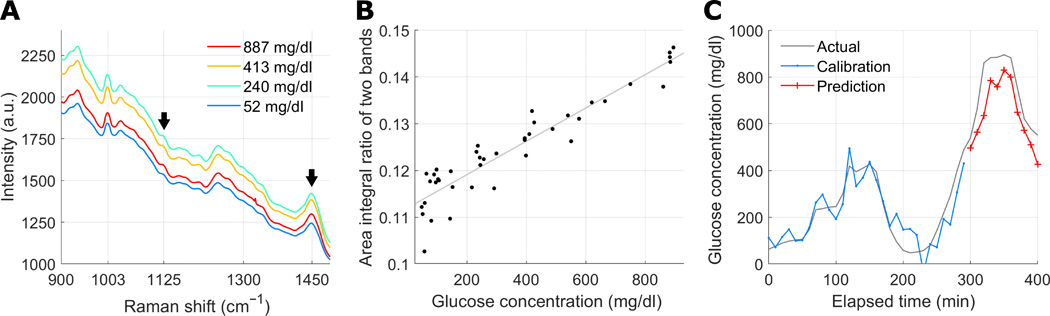
\includegraphics[width=3in]{figures/bloodGlucose-relative1125-directGlucose.jpeg}}\label{fig:bloodGlucose-relative1125-directGlucose}
    % \small{\textit{Note.} Additional notes goes here.}
\end{figure}

There are primarily two preprocessing options. 
Either extracting the features or utilize the complete Raman spectrum as an input.
The full spectrum analysis pair with partial least squares (PLS) is widely used \citep{forearm2014, sitecompare, forearm2005, directGlucose}.
The results vary from $R^2 = 0.62$ \citep{directGlucose}, $R^2 = 0.83$ \citep{forearm2005,forearm2014}, and RMSE of around 65 $\pm$ 0.4 ml/dL in~\cite{sitecompare}.
The preprocessing can be done by hand-pick \citep{directGlucose,solutionGlucose} or automatically \citep{ramanNailFold2019, sitecompare} pick the features.
Hand-pick features were performed by normalizing the spectra with either protein and lipid peaks (1450 $\text{cm}^{-1}$) \citep{directGlucose} or hemoglobin peaks (1549 $\text{cm}^{-1}$) \citep{solutionGlucose}.
It is demonstrated that the normalized 1125 $\text{cm}^{-1}$ has a linear correlation with in vivo blood glucose at $R^2 = 0.95$ \citep{solutionGlucose}.
In~\cite{directGlucose}, normalized 911, 1060, 1125 $\text{cm}^{-1}$ with 1450 $\text{cm}^{-1}$ were utilized as inputs of the more complex multiple linear regression (MLR) which achieved $R^2 = 0.91$.
The automatic feature extraction was demonstrated with PCA \citep{ramanNailFold2019} and SOM \citep{sitecompare}.



% Modeling the data with multiple linear regression (MLR) + hand-pick features (911, 1060, 1125, 1450 $\text{cm}^{-1}$) result in prediction correlation $R = 0.85$ for intrasubject cross-validation (CV) and $R = 0.91$ for intersubject CV \citep{directGlucose}.
% Full spectrum analysis using partial least squares (PLS) \citep{forearm2014, sitecompare, forearm2005, directGlucose} is widely used, and a few neural network approach \citep{ramanNailFold2019, sitecompare}.
% However, comparing model performance is difficult since each paper employs a different preprocessing technique.
% For a wearable with power and battery constraints, the suited model should provide good prediction accuracy (over 80\% of Clarke error grid (CEG) zone A) with low usage of resources.


% In glucose solution, the concentration of 0.1 - 40 mmol/L of glucose in water and Raman shift at 1125 $\text{cm}^{-1}$ has a linear relationship \cite{solutionGlucose}.
% The same case can not be said with blood glucose.
% Since blood contains multiple components, using 1125 $\text{cm}^{-1}$ directly will not work. 
% \cite{directGlucose} shows that the ratio of 1125 and 1450 (protein/lipid peak) $\text{cm}^{-1}$ yield a linear relationship.
% Figure~\ref{fig:bloodGlucose-relative1125} shows that the normalized 1125 $\text{cm}^{-1}$ has a linear relationship with the glucose concentration.
% This same procedure is also presented in \citep{solutionGlucose} where 1549 $\text{cm}^{-1}$ is used to normalize the spectrum.
% On the other hand, \cite{ramanNailFold2019} uses PCA and BP-ANN with an input layer of 3, a hidden layer of 4, and an output layer of 1. 
% While the model achieved an RMSE of 0.27 in intersubject modeling, using PCA is not necessarily means the features in use is a glucose-related feature \citep{directGlucose}.
% Adding to the neural network, FFNN is primarily used in modeling glucose in \citep{sitecompare}. 
% Without any feature selection, the RMSE of glucose prediction is 3.1 mmol/L and 30.12 mmol after implementing SOM and RReliefF as automatic feature selection.


%%%%%%%%%%%%%%%%%%%%%%%%%
% \section{Concentration Limitation}

% The usual blood glucose range of a healthy person can be as low as 0.3 - 1 mmol/L and $<$3 mmol/L for diabeties \citep{solutionGlucose}.



%%%%%%%%%%%%%%%%%%%%%%%%


% \begin{equation}
%     y = mx+b
% \end{equation}

% \begin{table}[]
% \caption{An example table in latex.}
% \begin{center}
% \begin{tabular}{l l}
% \hline
%     Methods & Metric\\ \hline
% Method A      & 153.3                \\ 
% Method B & 2.4                  \\ \hline
% \end{tabular}
% \label{tab:dense}
% \end{center}
% \small{\textit{Note.} Add notes here.}
% \end{table}
